\documentclass[10pt,twocolumn]{article}

\usepackage[letterpaper,margin=0.68in]{geometry}
\usepackage[utf8]{inputenc}
\usepackage{microtype}
\microtypesetup{expansion=false}
\usepackage{amsmath,amssymb}
\usepackage{booktabs}
\usepackage{graphicx}
\usepackage{xcolor}
\usepackage{tikz}
\usepackage{cite}
\usepackage{url}
\usepackage{xspace}
\usepackage{balance}
\usepackage[hidelinks]{hyperref}

\usetikzlibrary{arrows.meta,positioning,fit}

\setlength{\columnsep}{0.22in}
\addtolength{\textheight}{2pt}
\setlength{\parindent}{1em}
\setlength{\parskip}{0pt}
\setlength{\textfloatsep}{10pt plus 2pt minus 2pt}
\setlength{\floatsep}{9pt plus 2pt minus 2pt}
\renewcommand{\topfraction}{0.95}
\renewcommand{\bottomfraction}{0.90}
\renewcommand{\textfraction}{0.05}
\renewcommand{\floatpagefraction}{0.85}
\renewcommand{\dbltopfraction}{0.95}
\renewcommand{\dblfloatpagefraction}{0.85}
\setcounter{topnumber}{4}
\setcounter{dbltopnumber}{2}
\setcounter{totalnumber}{6}

\newcommand{\method}{\textsc{DCTPR}\xspace}
\newcommand{\datasetcub}{CUB-200-2011\xspace}
\newcommand{\datasetdogs}{Stanford Dogs\xspace}

\title{\method: Recovering Most Transductive Gains\\
with Three Support-Anchored Prototype Updates}
\author{Anonymous Authors}
\date{}

\begin{document}
\maketitle

\begin{abstract}
Frozen visual foundation models provide strong transferable representations,
but a single labeled image per class remains an unreliable prototype in
high-way fine-grained recognition. Transductive solvers can use the unlabeled
query set to correct this bias, although their iterative optimization can be
costly. We present Dual-Capacity Transductive Prototype Refinement
(\method), a training-free task adapter that concatenates normalized frozen
DINOv2-B/14 and DINOv2-L/14 features, estimates class-balanced query centers,
and performs three fixed prototype updates. We evaluate the frozen procedure
on three 200-way CUB episodes and three 120-way Stanford Dogs episodes, with
ten support rotations per episode. \method improves dual-capacity nearest
support classification by 6.68 and 6.27 percentage points on CUB and Dogs,
respectively. Its accuracy remains within 1.35 points of TIM-ADM on CUB and
0.61 points of MAP-RAW on Dogs, while its transductive head is 3.8 and 49 times
faster than those strongest matched solvers. Controlled class-imbalance tests
show that this efficiency depends materially on a known balanced query prior.
Relative to nearest support, \method recovers 83.3\% and 91.1\% of the accuracy
gain delivered by the strongest matched solver on CUB and Dogs. The results
position \method as a reproducible accuracy--efficiency operating point for
balanced, high-way, one-shot fine-grained recognition rather than as an
accuracy state-of-the-art method.
\end{abstract}

\noindent\textbf{Keywords:} few-shot learning; transductive inference;
fine-grained recognition; frozen visual foundation models; prototype refinement

\section{Introduction}
\label{sec:introduction}

Fine-grained recognition distinguishes visually similar categories while
remaining robust to pose, viewpoint, background, and within-class appearance
variation. These properties make the problem particularly sensitive to label
scarcity. When only one labeled image represents each class, the support image
is both the supervision signal and the initial class prototype. Atypical pose or
background content can therefore shift the prototype away from the query
distribution even when the underlying feature extractor is strong. Prior
fine-grained few-shot methods therefore devote explicit machinery to local
attention, feature reconstruction, or cross-image correspondence
\cite{mamlfgvc,dualattention,bfrn}.

Large self-supervised visual encoders such as DINOv2 provide transferable
representations without task-specific backbone training \cite{dinov2}. Their
strength changes the practical few-shot question. In a moderate-shot regime,
the representation and a simple classifier may already be difficult to improve,
as established by transfer-based and nearest-centroid studies
\cite{closerlook,goodembedding,simpleshot}.
In a high-way one-shot regime, however, the dominant error can instead arise
from estimating a class center from one observation. This distinction motivates
task-level adaptation that corrects prototypes without fitting neural parameters.

Transductive few-shot methods jointly classify an unlabeled query set and can
reduce single-support bias. LaplacianShot propagates information over a query
graph \cite{laplacianshot}; TIM optimizes a mutual-information objective
\cite{tim}; and PT-MAP combines feature transformation, optimal transport, and
prototype updates \cite{ptmap}. These methods establish strong accuracy
baselines, but their graph or iterative optimization also creates a practical
latency cost. Moreover, many transductive benchmarks assume that every class has
the same number of queries, an assumption that can strongly affect inference
\cite{realistictransduction}. The unresolved engineering question is therefore
not only which solver is most accurate, but how much of the transductive gain can
be recovered by a short, transparent, and training-free update under an explicit
query-prior scope.

This question calls for a different evaluation target from an accuracy-only
leaderboard. A useful short adapter should produce a substantial improvement
over the inductive reference, remain close to the strongest matched solver,
and reduce the task-level work required for every new episode. These three
requirements must be evaluated together. Reporting only the gain over nearest
support would hide the remaining accuracy gap, whereas reporting only the best
accuracy would hide the cost of reaching it. We therefore treat accuracy,
runtime, cross-episode stability, and prior sensitivity as parts of one
operating-point claim.

We address this question with Dual-Capacity Transductive Prototype Refinement
(\method). The method combines frozen DINOv2-B/14 and DINOv2-L/14 class-token
features, imposes the known balanced query marginal through a soft Sinkhorn
assignment, and alternates assignment with a support-anchored query-center
update for exactly three refinement steps. The procedure does not read query
labels and learns no task-specific parameters. It is evaluated under a frozen
development--confirmation protocol on CUB and then transferred without retuning
to Stanford Dogs.

Our contributions are threefold. First, we define a compact dual-capacity task
adapter for balanced high-way one-shot recognition and specify its assumptions,
normalization, assignment, and update rules completely. Second, we evaluate the
method across two fine-grained datasets, six train-only episodes, and 60 support
rotations against matched implementations of established transductive solvers.
Third, we report both computational cost and controlled query-imbalance stress
tests, establishing where the method is competitive and where its uniform-prior
assumption fails.

\section{Related Work}
\label{sec:related}

\subsection{Frozen representations for few-shot recognition}

Transfer-based few-shot learning often separates representation learning from
task inference. A strong encoder can make simple nearest-center or linear
classifiers competitive, which places a higher burden on any adaptation module
to show that its gain is not caused by a weak feature baseline
\cite{closerlook,goodembedding,simpleshot}. DINOv2 learns
general-purpose visual features through self-supervised pretraining
\cite{dinov2}. We therefore freeze both DINOv2 encoders in all experiments and
apply every compared transductive solver to the same extracted features. This
design isolates task inference from backbone optimization.

Fine-grained datasets add a complementary challenge: class identity can depend
on small appearance differences while nuisance variation dominates the image.
CUB \cite{cubdataset} and Stanford Dogs \cite{stanforddogs} are widely used to
study such distinctions, including in attention- and reconstruction-based
few-shot recognition \cite{mamlfgvc,dualattention,bfrn}. Rather than
constructing a conventional 5-way task,
we evaluate all available categories in each episode. This high-way setting
magnifies competition among similar categories and makes support-prototype bias
visible even with foundation-model features.

\subsection{Transductive inference and prototype correction}

Transductive methods use the query set jointly rather than predicting each query
independently. LaplacianShot optimizes unary support distances together with a
graph smoothness term \cite{laplacianshot}. TIM alternates classifier updates
under supervised support and query information objectives \cite{tim}. PT-MAP
applies a feature transform and Sinkhorn-based assignment before iteratively
moving class prototypes \cite{ptmap}. Related work also shows that careful
feature preprocessing and simple classifier ensembles can remain competitive
without episodic meta-training \cite{squeezefeatures,easy}. More recent work further combines graph
and prototype refinement \cite{iterativegraph} or learns conditional transport
for unknown query proportions \cite{conditionaltransport}.

\method does not claim the individual novelty of feature concatenation,
Sinkhorn normalization, or prototype refinement. Its contribution is the scoped
combination of complementary frozen capacities with a deliberately short update
schedule, together with a matched high-way accuracy--efficiency evaluation. The
method is consequently compared against the established solver families on the
same feature tensors instead of against a weaker classifier alone.

\subsection{Query priors in transductive evaluation}

Balanced query sets provide useful controlled evaluation, but they also reveal
the class marginal to the inference procedure. Veilleux et al. showed that
methods encoding a uniform marginal can degrade under Dirichlet-distributed
query proportions and proposed an alpha-entropy objective to reduce this bias
\cite{realistictransduction}. Conditional transport and adaptive-manifold
methods subsequently targeted imbalanced transduction directly
\cite{conditionaltransport,adaptivemanifold}. We treat balance as an explicit
assumption rather than a hidden property. Our primary experiments test the
balanced high-way setting, while separate mild and severe imbalance regimes
measure how far the conclusion extends.

\section{Method}
\label{sec:method}

\subsection{Task formulation}

An episode contains $C$ classes and one labeled support image per class,
$\mathcal{S}=\{(x_c^s,c)\}_{c=1}^{C}$. The unlabeled query set is
$\mathcal{Q}=\{x_i^q\}_{i=1}^{N}$. In the primary protocol, each class occurs
exactly $q=N/C$ times in $\mathcal{Q}$, but query labels are never observed by
the method. The goal is to predict all query labels jointly using frozen image
features and the known balanced column mass $q$.

Figure~\ref{fig:pipeline} summarizes \method. Two frozen encoders produce
complementary image representations. The fused support features initialize the
class prototypes. Each refinement step alternates a balanced soft assignment
with a support-anchored query-center update. The final assignment provides the
query predictions.

\begin{figure*}[!t]
\centering
\resizebox{\textwidth}{!}{%
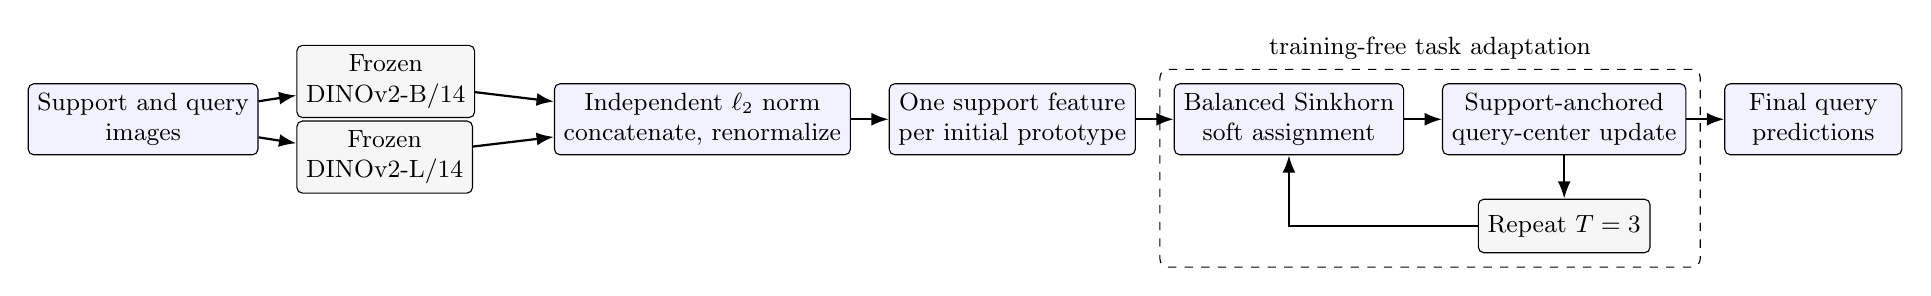
\begin{tikzpicture}[
  node distance=0.55cm and 0.48cm,
  block/.style={draw, rounded corners=2pt, align=center, minimum height=0.78cm,
                minimum width=2.25cm, fill=blue!5, font=\small},
  smallblock/.style={draw, rounded corners=2pt, align=center, minimum height=0.68cm,
                minimum width=1.95cm, fill=gray!7, font=\small},
  arrow/.style={-{Latex[length=2.2mm]}, thick},
  group/.style={draw, dashed, rounded corners=3pt, inner sep=5pt}
]
\node[block] (images) {Support and query\\images};
\node[smallblock, right=of images, yshift=0.48cm] (b) {Frozen\\DINOv2-B/14};
\node[smallblock, right=of images, yshift=-0.48cm] (l) {Frozen\\DINOv2-L/14};
\node[block, right=1.0cm of b, yshift=-0.48cm] (fusion) {Independent $\ell_2$ norm\\concatenate, renormalize};
\node[block, right=of fusion] (proto) {One support feature\\per initial prototype};
\node[block, right=of proto] (assign) {Balanced Sinkhorn\\soft assignment};
\node[block, right=of assign] (update) {Support-anchored\\query-center update};
\node[smallblock, below=0.55cm of update] (repeat) {Repeat $T=3$};
\node[block, right=of update] (predict) {Final query\\predictions};
\draw[arrow] (images) -- (b);
\draw[arrow] (images) -- (l);
\draw[arrow] (b) -- (fusion);
\draw[arrow] (l) -- (fusion);
\draw[arrow] (fusion) -- (proto);
\draw[arrow] (proto) -- (assign);
\draw[arrow] (assign) -- (update);
\draw[arrow] (update) -- (predict);
\draw[arrow] (update) -- (repeat);
\draw[arrow] (repeat.west) -| (assign.south);
\node[group, fit=(assign)(update)(repeat), label={[font=\small]above:training-free task adaptation}] {};
\end{tikzpicture}
}
\caption{Overview of \method. Both encoders remain frozen. The method uses the
balanced query marginal but never accesses query labels. Only the assignment
and support-anchored prototype update are repeated.}
\label{fig:pipeline}
\end{figure*}

\subsection{Design principles}

\method is designed around four constraints. First, all task information must
enter through the support and unlabeled query features; the adapter must not
update either encoder or learn task-specific neural parameters. Second, the
support example must remain an explicit anchor because the initial soft
assignments can contain errors. Third, the query-set constraint must match an
assumption that can be stated and tested, rather than silently exploiting a
balanced sampler. Fourth, task-level computation must be bounded by a small
fixed number of matrix operations.

These constraints determine the pipeline in Figure~\ref{fig:pipeline}.
Independent normalization prevents the larger feature family from contributing
only through scale. Balanced assignment uses the known query marginal to
regularize an otherwise uncertain 200- or 120-way matching problem.
Support-anchored updates incorporate the resulting query centers without
recursively replacing the labeled evidence. Finally, fixing the schedule to
three updates makes latency independent of a convergence tolerance. The
component study tests the first three choices, while the matched runtime
comparison tests whether the short schedule produces a useful operating point.

\subsection{Dual-capacity representation}

Let $f_B(x)\in\mathbb{R}^{d_B}$ and
$f_L(x)\in\mathbb{R}^{d_L}$ denote the class-token outputs of frozen DINOv2-B/14
and DINOv2-L/14. Each capacity is normalized before concatenation so that one
feature family cannot dominate only because of its raw norm:
\begin{equation}
 \bar f_k(x)=\frac{f_k(x)}{\lVert f_k(x)\rVert_2},\qquad k\in\{B,L\}.
\end{equation}
The fused representation is
\begin{equation}
 z(x)=\frac{[\bar f_B(x);\bar f_L(x)]}
 {\lVert[\bar f_B(x);\bar f_L(x)]\rVert_2}.
 \label{eq:fusion}
\end{equation}
The initial prototype is the only labeled representation for its class,
$p_c^{(0)}=z(x_c^s)$. The ablation in Section~\ref{sec:ablation} tests whether
the fused representation contributes beyond either capacity alone.

\subsection{Balanced soft assignment}

At refinement step $t$, cosine logits compare every query with every prototype:
\begin{equation}
 A_{ic}^{(t)}=\frac{z(x_i^q)^\top p_c^{(t)}}{\tau},
 \qquad \tau=0.05.
 \label{eq:logits}
\end{equation}
We exponentiate the stabilized logits and apply Sinkhorn row and column scaling
\cite{sinkhorn}. The resulting matrix $P^{(t)}\in\mathbb{R}_+^{N\times C}$
satisfies
\begin{equation}
 P^{(t)}\mathbf{1}_{C}=\mathbf{1}_{N},\qquad
 (P^{(t)})^\top\mathbf{1}_{N}=q\mathbf{1}_{C}.
 \label{eq:marginals}
\end{equation}
The row constraint produces a categorical distribution for each query, while
the column constraint encodes the known balanced query count. We use 100
normalization iterations. Equation~\eqref{eq:marginals} is a task assumption,
not a learned estimate; Section~\ref{sec:priorstress} tests its failure under
unknown non-uniform counts.

\subsection{Support-anchored prototype update}

The soft query center for class $c$ is
\begin{equation}
 \mu_c^{(t)}=\frac{\sum_{i=1}^{N}P_{ic}^{(t)}z(x_i^q)}
 {\sum_{i=1}^{N}P_{ic}^{(t)}}.
 \label{eq:center}
\end{equation}
We anchor every update to the original labeled support rather than recursively
averaging the preceding prototype:
\begin{equation}
 p_c^{(t+1)}=\operatorname{norm}_2\left(
 (1-\lambda)p_c^{(0)}+\lambda\mu_c^{(t)}\right),
 \qquad \lambda=0.5.
 \label{eq:update}
\end{equation}
The assignment and update are repeated for $T=3$ steps, after which a final
balanced assignment yields the predicted class. This support anchor limits
prototype drift, while the short fixed schedule bounds task-level latency.
No gradient update, query label, or dataset-specific parameter is used after the
CUB development episode.

For feature dimension $d=d_B+d_L$, one assignment/update step is dominated by
the $N\times C$ similarity matrix and query-center aggregation, both
$O(NCd)$. The Sinkhorn normalization acts on the smaller assignment matrix. In
our implementation, the complete three-step transductive head takes about
33--34 ms per high-way support rotation on an RTX 3080 Ti, excluding the common
frozen feature extraction stage.

\section{Experimental Protocol}
\label{sec:protocol}

\subsection{Datasets and episode construction}

\datasetcub contains 200 bird species \cite{cubdataset}. Each CUB episode uses
ten official-training images per class, producing a 200-way task with one
support and nine queries per class. Three episodes are evaluated. Episode 1 is
the only development episode; Episodes 2 and 3 are confirmation episodes.

\datasetdogs contains 120 dog breeds \cite{stanforddogs}. We select three
pairwise-disjoint groups of ten images per class from the official training
list, for 3,600 unique images in total. Each group defines a 120-way one-shot
episode with nine queries per class. All method and baseline constants are
transferred from CUB without using Dogs labels for selection.

Figure~\ref{fig:training-examples} illustrates the task: related classes can
differ in subtle plumage or shape while pose and background vary substantially.

\begin{figure*}[!t]
\centering
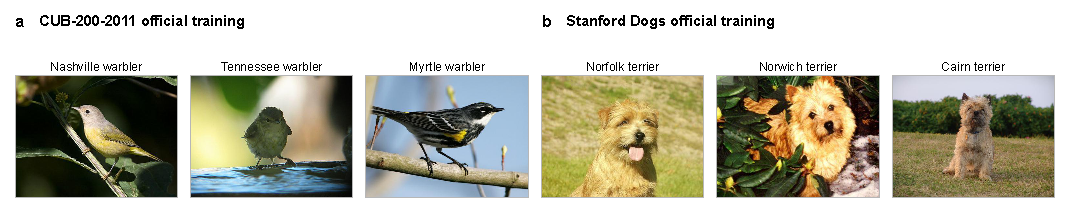
\includegraphics[width=\textwidth]{../figures/fig_training_examples.pdf}
\caption{\textbf{Official-training examples.} \textbf{a}, CUB-200-2011
warblers. \textbf{b}, Visually similar Stanford Dogs terriers. This
context-only plate is not quantitative evidence. Images were split-verified
and center-cropped without color or contrast adjustment; no official-test
image is shown.}
\label{fig:training-examples}
\end{figure*}

Within each episode, the ten images of every class take turns as support. This
produces ten paired rotations and ensures that every image is used as the sole
support once. We report the mean balanced accuracy across rotations. Because
rotations reuse episode images, their standard deviations are descriptive and
are not treated as independent-sample confidence intervals. No CUB or Dogs
official-test image was decoded or encoded during this study.

\subsection{Features and implementation}

Images are directly resized to $392\times392$. We extract the class token from
the official frozen DINOv2 ViT-B/14 and ViT-L/14 models. The same saved feature
tensors are supplied to all inference methods. \method uses $\tau=0.05$, 100
Sinkhorn normalizations, $T=3$ prototype updates, and $\lambda=0.5$. These
constants are frozen before CUB confirmation and before all Dogs experiments.

Runtime is measured only for the task-level transductive head on one NVIDIA
GeForce RTX 3080 Ti; common feature extraction and disk loading are excluded.
The reported time is the mean wall-clock duration per support rotation, with
CUDA synchronization around the measured call.

\subsection{Matched baselines}

The inductive reference, BL nearest support (BL-NCC), predicts from cosine
similarity in the fused feature space. BL-Sinkhorn adds balanced soft assignment
without prototype refinement. Single-capacity refinement applies the same update
to either B or L features.

We additionally implement TIM-ADM \cite{tim}, raw MAP and signed-power PT-MAP
\cite{ptmap}, and LaplacianShot \cite{laplacianshot}. Their published update
rules are applied to the common DINO features. TIM-ADM uses temperature 15,
loss weights $(0.1,1.0,0.1)$, 150 alternating updates, and update factor 1.
MAP uses transport regularization 10, prototype update factor 0.2, and 20
updates. Since DINO class-token values are signed, the PT-MAP power-transform
arm uses an explicitly labeled signed square-root adaptation. LaplacianShot
uses directed non-self neighbors, 20 bound updates, and a published lambda grid
selected only on CUB Episode 1. These are matched feature-level
reimplementations, not executions of the original end-to-end backbone pipelines.

\subsection{Metrics and comparison logic}

Balanced accuracy is the primary metric because every primary episode has the
same number of queries per class and the stress test deliberately changes those
counts. For the balanced episodes, balanced accuracy equals ordinary query
accuracy. For the imbalanced regimes, we compute recall per class and average
over classes so that frequent classes cannot dominate the result.

Runtime measures only the task-level transductive head. This isolates the
computational difference among solvers because all methods receive the same
saved DINOv2 features. It does not measure end-to-end image latency and should
not be interpreted as such. BL-NCC has zero additional task-head optimization
and is therefore reported as an inductive reference rather than placed at an
artificial positive time on logarithmic plots.

To summarize how much of the strongest solver's improvement is retained, we
also report a descriptive gain-recovery ratio
\begin{equation}
 R_{\mathrm{gain}}=
 \frac{A_{\method}-A_{\mathrm{BL}}}
 {A_{\mathrm{strong}}-A_{\mathrm{BL}}},
 \label{eq:recovery}
\end{equation}
where $A_{\mathrm{strong}}$ is the accuracy of the strongest matched
transductive solver on that dataset. This ratio complements, rather than
replaces, the absolute accuracy and runtime values.

\section{Results}
\label{sec:results}

\subsection{Component analysis}
\label{sec:ablation}

Table~\ref{tab:ablation} separates capacity fusion, balanced assignment, and
prototype refinement. BL-NCC averages 68.17\% across CUB. Balanced assignment
without refinement raises this to 73.50\%, showing that query-set geometry
provides most of the initial gain. Refinement on B or L alone reaches 73.40\%
and 73.20\%, respectively. Combining both capacities with assignment and
support-anchored updates reaches 74.85\%, 1.35 points above BL-Sinkhorn and
1.45--1.65 points above the single-capacity refinements.

\begin{table}[t]
\centering
\caption{CUB component analysis. Values are balanced accuracy (\%) averaged
over ten rotations. E1 is development; E2--E3 are frozen confirmation.}
\label{tab:ablation}
\resizebox{\columnwidth}{!}{%
\begin{tabular}{lrrrr}
\toprule
Method & E1 & E2 & E3 & Mean \\
\midrule
BL nearest support & 68.42 & 68.12 & 67.96 & 68.17 \\
B-only refinement & 73.84 & 73.22 & 73.13 & 73.40 \\
L-only refinement & 73.46 & 73.22 & 72.92 & 73.20 \\
BL balanced assignment & 73.79 & 73.44 & 73.26 & 73.50 \\
\textbf{DCTPR} & \textbf{75.14} & \textbf{74.71} & \textbf{74.69} & \textbf{74.85} \\
\bottomrule
\end{tabular}}
\end{table}

The frozen confirmation is important because Episode 1 determined the fixed
method constants. On Episodes 2 and 3, \method exceeds the strongest component
comparator by 1.27 and 1.43 points, respectively, while improving over BL-NCC
by 6.59 and 6.73 points. Thus the full configuration does not depend on the
development episode alone.

We also screened an agreement-weighted consensus extension on Episode 1. It
reached 75.18\%, only 0.04 points above its paired refinement reference, and was
non-inferior in 6 of 10 rotations. It failed the frozen development gate and was
not retained. This negative control favors the simpler fixed \method update over
an unconfirmed adaptive weighting mechanism.

\subsection{Accuracy--efficiency comparison}

Table~\ref{tab:main} compares established transductive solvers using the same
features and episodes. On CUB, TIM-ADM is the most accurate method at 76.19\%.
\method reaches 74.85\%, a deficit of 1.35 points, but takes 33.3 ms rather
than 126.3 ms per rotation, a 3.8-fold reduction. \method also exceeds both MAP
arms and the LaplacianShot variants on CUB.

On Dogs, MAP-RAW is strongest at 70.97\%, while \method reaches 70.36\%.
The 0.61-point difference is accompanied by a substantial runtime difference:
34.1 ms for \method and 1,678.6 ms for MAP-RAW, or approximately 49-fold.
\method is also 0.36 points above TIM-ADM on Dogs while remaining about four
times faster. These comparisons support an accuracy--efficiency claim, but not
an accuracy state-of-the-art claim.

\begin{table*}[!t]
\centering
\caption{Matched transductive comparison. Accuracy is the mean balanced
accuracy across three episodes and 30 rotations per dataset. Runtime is mean
milliseconds per rotation for the transductive head only. Bold marks the best
accuracy; underlining marks \method.}
\label{tab:main}
\begin{tabular}{lrrrr}
\toprule
& \multicolumn{2}{c}{CUB, 200-way} & \multicolumn{2}{c}{Stanford Dogs, 120-way} \\
\cmidrule(lr){2-3}\cmidrule(lr){4-5}
Method & Accuracy (\%) & Runtime (ms) & Accuracy (\%) & Runtime (ms) \\
\midrule
BL nearest support & 68.17 & 0.0 & 64.09 & 0.0 \\
BL balanced assignment & 73.50 & 10.9 & 66.88 & 12.0 \\
LaplacianShot & 68.30 & 2.2 & 64.43 & 3.9 \\
MAP-RAW & 74.30 & 1,612.9 & \textbf{70.97} & 1,678.6 \\
Signed PT-MAP adaptation & 74.37 & 1,612.5 & 70.94 & 1,666.0 \\
TIM-ADM & \textbf{76.19} & 126.3 & 70.01 & 139.2 \\
\underline{\method} & \underline{74.85} & \underline{33.3} & \underline{70.36} & \underline{34.1} \\
\bottomrule
\end{tabular}
\end{table*}

Figure~\ref{fig:pareto} makes the operating-point comparison explicit. On CUB,
\method lies between the inexpensive balanced assignment and the more accurate
TIM-ADM solver. It recovers
$(74.85-68.17)/(76.19-68.17)=83.3\%$ of TIM-ADM's gain over BL-NCC while using
26.4\% of its task-head runtime. On Dogs, it recovers
$(70.36-64.09)/(70.97-64.09)=91.1\%$ of MAP-RAW's gain while using 2.0\% of its
runtime. The result is therefore not merely that \method is faster than the
most accurate comparator. It retains most of that comparator's improvement
over the same inductive reference.

\begin{figure*}[!t]
\centering
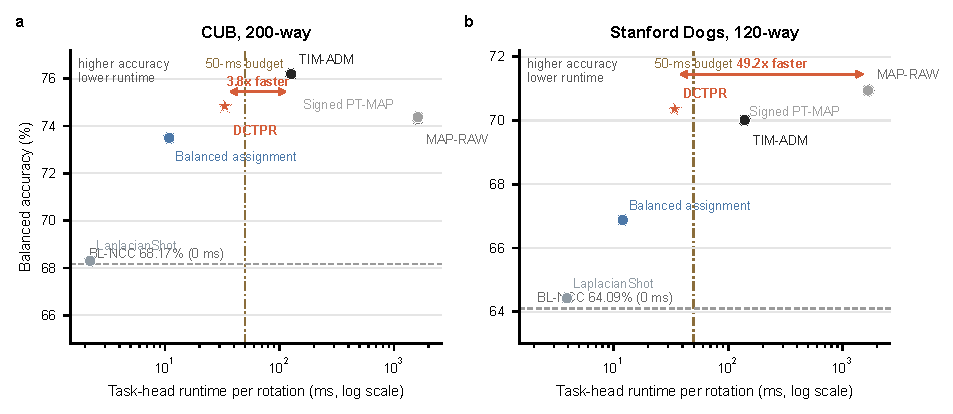
\includegraphics[width=\textwidth]{../figures/fig2_accuracy_efficiency.pdf}
\caption{\textbf{Accuracy--efficiency operating points on two high-way
datasets.} \textbf{a}, CUB-200-2011, evaluated as 200-way one-shot
classification. \textbf{b}, Stanford Dogs, evaluated as 120-way one-shot
classification. Each point reports mean balanced accuracy and mean task-head
runtime across three episodes and 30 support rotations. All methods use the
same saved DINOv2 features. The dashed horizontal line is the zero-optimization
BL-NCC reference and is not assigned an artificial value on the logarithmic
runtime axis. DCTPR is 3.8 times faster than TIM-ADM on CUB and 49.2 times
faster than MAP-RAW on Dogs.}
\label{fig:pareto}
\end{figure*}

\subsection{Cross-episode and cross-dataset stability}

The gain over nearest support is consistent across all six episodes
(Table~\ref{tab:episodes}). CUB gains range from 6.59 to 6.73 points. Dogs gains
range from 5.94 to 6.58 points even though no Dogs label informed method or
baseline selection. All 30 Dogs support rotations improve over BL-NCC. The
similar gain magnitude across a bird dataset and a dog-breed dataset suggests
that the method is correcting a recurring one-shot prototype problem rather
than only exploiting one CUB episode construction.

The rotation-level view in Figure~\ref{fig:robustness}a strengthens this
descriptive result. Every one of the 60 paired rotations improves over BL-NCC,
despite different support images and disjoint episode image groups. The
dispersion is wider within episodes than the variation among episode means:
individual gains range from approximately four to nine points, whereas the six
episode means remain between 5.94 and 6.73 points. Because rotations reuse
images, these points are evidence of paired stability rather than independent
replicates for a significance test.

\begin{table}[t]
\centering
\caption{Per-episode stability of the gain over fused nearest support.}
\label{tab:episodes}
\begin{tabular}{lrrr}
\toprule
Dataset/episode & BL-NCC & \method & Gain (pp) \\
\midrule
CUB E1 & 68.42 & 75.14 & +6.72 \\
CUB E2 & 68.12 & 74.71 & +6.59 \\
CUB E3 & 67.96 & 74.69 & +6.73 \\
Dogs E1 & 63.78 & 69.72 & +5.94 \\
Dogs E2 & 64.46 & 71.05 & +6.58 \\
Dogs E3 & 64.04 & 70.32 & +6.29 \\
\bottomrule
\end{tabular}
\end{table}

\subsection{Query-prior stress test}
\label{sec:priorstress}

The primary protocol supplies the exact class-balanced column mass used by
Equation~\eqref{eq:marginals}. We test the consequence of violating this
assumption on CUB. In the mild regime, half the classes retain three queries and
half retain nine. In the severe regime, class counts range from one to nine.
Counts are permuted across classes with fixed seeds, and macro balanced accuracy
prevents majority classes from dominating the metric.

Table~\ref{tab:stress} shows that uniform-prior \method falls to 68.34\% and
68.86\%, close to nearest support and below its balanced-query result. Replacing
the uniform marginal with true class counts, solely as an oracle diagnostic,
recovers 73.35\% and 72.87\%. The 4.01--5.01 point mean gaps indicate that
incorrect class mass, rather than complete loss of query geometry, explains a
large fraction of the degradation. Oracle counts are never used as a deployable
method input.

\begin{table}[t]
\centering
\caption{CUB macro balanced accuracy (\%) under deterministic query imbalance,
averaged over three episodes. Oracle counts are diagnostic only.}
\label{tab:stress}
\resizebox{\columnwidth}{!}{%
\begin{tabular}{lrr}
\toprule
Method & Mild 3/9 & Severe 1--9 \\
\midrule
BL nearest support & 68.33 & 68.19 \\
TIM-ADM & \textbf{70.31} & 68.94 \\
\method, uniform prior & 68.34 & 68.86 \\
\method, oracle counts & 73.35 & \textbf{72.87} \\
\bottomrule
\end{tabular}}
\end{table}

\begin{figure*}[!t]
\centering
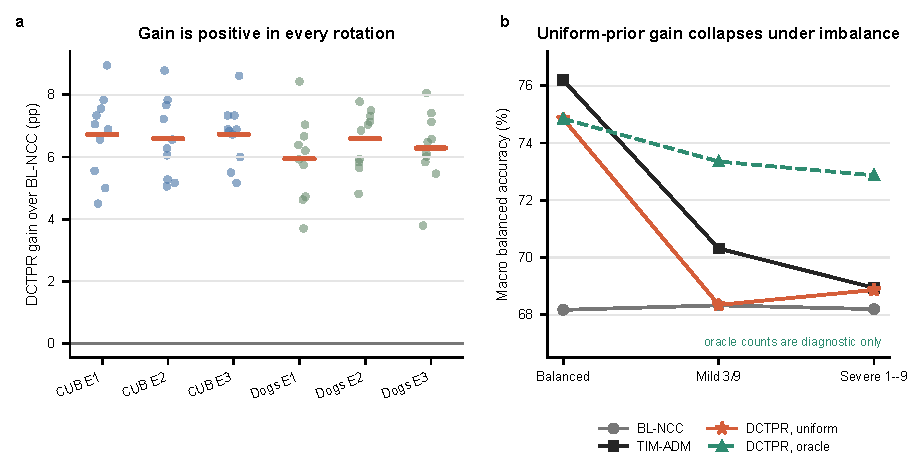
\includegraphics[width=\textwidth]{../figures/fig3_stability_prior.pdf}
\caption{\textbf{Stable one-shot gains and their query-prior boundary.}
\textbf{a}, Paired DCTPR gain over BL-NCC for each support rotation. Dots are
the ten rotations per episode and orange bars are episode means; rotation
dispersion is descriptive because rotations reuse images. All 60 differences
are positive. \textbf{b}, Mean CUB macro balanced accuracy across the balanced
protocol and two deterministic imbalance regimes. Uniform-prior DCTPR loses
most of its balanced-task advantage, whereas supplying the true class counts
recovers much of the loss. Oracle counts are a diagnostic and are never used as
a deployable method input.}
\label{fig:robustness}
\end{figure*}

Figure~\ref{fig:robustness}b places the stress result next to the balanced
operating point. The uniform and oracle DCTPR curves coincide when the query set
is balanced because the assumed and true class marginals are identical. They
separate immediately when the class counts become non-uniform. This pattern
localizes the failure to the marginal constraint: query features still contain
recoverable information, but the uniform column mass allocates that information
to the wrong class totals.

\section{Discussion}
\label{sec:discussion}

The central result is not maximum accuracy, but that short support-anchored
refinement recovers a large and stable fraction of the gap between nearest
support and stronger optimization. Component analysis attributes this to
balanced assignment, which corrects much of the single-support bias, and
dual-capacity refinement, which adds 1.35 points. Both single-capacity variants
are weaker than the fusion, although this does not establish a causal semantic
mechanism.

The gain-recovery view clarifies the magnitude of this result. On the two
datasets, the three-step adapter retains 83.3--91.1\% of the improvement that
the strongest matched solver obtains over nearest support. This is more
informative than comparing \method only with BL-NCC, because it accounts for
the accuracy still available from heavier optimization. It is also more
conservative than calling the method Pareto-optimal in a universal sense: the
frontier depends on the evaluated solver set, hardware, feature tensors, and
episode construction.

The runtime comparison defines the useful operating regime. TIM-ADM adds 1.35
points on CUB at 3.8 times the task-head runtime; MAP-RAW adds 0.61 points on
Dogs at about 49 times the runtime. Maximum-accuracy offline use may prefer
those solvers, whereas repeated support selection or interactive recognition
can amortize feature extraction and benefit from the three-step head. This is
an engineering tradeoff, not universal dominance, and it does not imply that
head latency dominates end-to-end image encoding.

The dual-capacity result should also be interpreted narrowly. Fusion improves
over both single-capacity refinements on all three CUB episodes, and the frozen
configuration transfers to Dogs without retuning. This is consistent with
useful geometric complementarity between the B and L representations.
Nevertheless, concatenation increases stored feature dimensionality, and the
experiments do not identify which semantic attributes are complementary.
Accordingly, dual capacity is supported as an empirical design choice within
the adapter, not as a demonstrated representation mechanism.

The balanced query prior is the main scope limitation. Under both imbalance
regimes, forcing uniform class mass removes most of the balanced-task advantage.
This agrees with broader evidence that class-balanced transductive benchmarks
can favor methods that encode a uniform marginal \cite{realistictransduction}.
Future extensions should estimate class proportions without query labels and
should be evaluated on public Dirichlet-imbalance protocols against specialized
methods such as conditional transport and adaptive manifolds
\cite{conditionaltransport,adaptivemanifold}. Such an extension is separate
from the balanced-prior claim established here.

Three additional boundaries affect interpretation. First, the episodes use
official training partitions to preserve an untouched official test; the
reported numbers are therefore controlled train-only protocol results rather
than standard leaderboard results. Second, established baselines are matched
reimplementations of their update rules on common DINO features, not full
executions of their original pretrained pipelines. Third, support rotations
share images, so rotation variability is descriptive. These choices strengthen
paired control and reproducibility but limit direct comparison with published
results under different backbones, splits, and task samplers.

Two evaluations are therefore needed before extending the claim: a public
imbalanced protocol with estimated class proportions and matched backbones, and
end-to-end latency measurements across hardware and batch sizes. They would
test whether the short-update advantage survives unknown marginals and image
encoding, respectively.

\section{Conclusion}
\label{sec:conclusion}

We introduced \method, a training-free dual-capacity adapter for balanced,
high-way, one-shot fine-grained recognition. Across CUB and Stanford Dogs, the
method improves fused nearest-support classification by 6.68 and 6.27
percentage points, respectively, while remaining within 0.61--1.35 points of
the strongest matched transductive solvers at substantially lower task-level
runtime. Equivalently, it retains 83.3--91.1\% of the strongest solver's gain
over nearest support while using 2.0--26.4\% of that solver's runtime.
Component and frozen cross-dataset results support the use of short
support-anchored query-center refinement as a practical accuracy--efficiency
choice. The conclusion is explicitly bounded by a known balanced query prior;
controlled imbalance tests show that removing this assumption requires a
different inference design.

\section*{Reproducibility Statement}

The project archive contains immutable experiment protocols, feature metadata,
per-rotation predictions, summary JSON files, source hashes, and independent
recomputation reports. Both quantitative figures are reconstructed from those
archives, and the image plate uses six split-verified, hashed training samples.
Figure source-data CSV files and the Python generation script accompany the
draft. All method constants are stated in Sections~\ref{sec:method} and
\ref{sec:protocol}, and all official-test access counters remain zero.

\bibliographystyle{unsrt}
{\fontsize{7.5pt}{8.5pt}\selectfont\bibliography{references}}

\end{document}
